\documentclass{article}
\usepackage[english]{babel}
\usepackage[a4paper,top=2cm,bottom=2cm,left=2cm,right=2cm,marginparwidth=1.75cm]{geometry}
\usepackage{tikz}
\usetikzlibrary{automata, positioning, arrows}
\title{ Tecnológico de Costa Rica \\
Escuela de Ingeniería en Computación\\
Teoría de Automatas y Lenguajes Formales \\
II Sem - 2023 \\
Proyecto Programado 1
}\author{
Daniel Amador Salas\\
\texttt{2017022096}
\and
Sebastián Francisco Gamboa Chacóns\\
\texttt{2017142512}
\and
Gerardo Gutierrez Quirós\\
\texttt{2016140286}
\and
Josef Ruzicka González\\
\texttt{2024800833}
}
\date{}
\begin{document}
\maketitle
\section{Definición Formal}
Un DFA se define como el siguiente quinteto:\begin{equation}
M = (Q, \sum, \delta, q_0, F)\
\end{equation}
\subsection{Q}
Es el conjunto de estados finitos.\\En nuestro ejemplo este conjunto está dado por: 
\begin{equation}
 \{1, 2, 3\}
\end{equation}
\subsection{$\sum$}
Es el alfabeto.\\En nuestro ejemplo este conjunto está dado por: 
\begin{equation}
 \{a, b, c\}
\end{equation}
\subsection{$\delta$}
Es la función de transición. La podemos representar como una tabla donde las filas son los estados y las columnas los símbolos del alfabeto.\\
 Formalmente se representa como el siguiente producto cartesiano:\begin{equation}
\delta: Q x \sum
\end{equation}
En nuestro ejemplo esta tabla corresponde a: 
\begin{center}
\begin{tabular}{c c c c }
 & a & b & c\\
1 & 3 & 2 & 1\\
2 & - & 2 & 1\\
3 & - & - & 1\\
\end{tabular}\end{center}\subsection{$q_0$}
Es el estado inicial.\\En nuestro ejemplo el estado inicial es: \
 1\subsection{F}
Es el conjunto de estados de aceptación.\\En nuestro ejemplo este conjunto está dado por: 
\begin{equation}
 \{3, \}
\end{equation}
\section{Grafo del DFA}
\tikzset{ 
 ->, >=stealth, node distance=3cm
}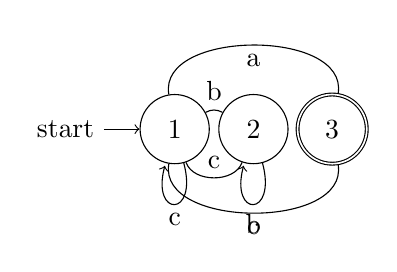
\begin{tikzpicture}
\node[state, initial] (0) {$1$};
\node[state, , right of=0] (1) {$2$};
\node[state, accepting, right of=1] (2) {$3$};
\draw (0) edge[bend left=3.50cm, below] node {a} (2)
(0) edge[bend left=1.0cm, above] node {b} (1)
(0) edge[loop below] node{c} (0) 
(1) edge[loop below] node{b} (1) 
(1) edge[bend left=2.50cm, above] node {c} (0)
(2) edge[bend left=3.50cm, below] node {c} (0)
;
\end{tikzpicture}
\section{Ejemplos de Hileras Aceptadas}
\begin{equation}
\{
ca,ccca,cccaca,bbbcca,a,\}
\end{equation}
\section{Ejemplos de Hileras Rechazadas}
\begin{equation}
\{
c,cbbac,cbba,bcaa,bcaaa,\}
\end{equation}
\section{ Regex - Teorema de Arden}
\subsection{ Ecuaciones de Estado}
\begin{equation}
1 = \epsilon + 1c+ 2c+ 3c
\end{equation}
\begin{equation}
2 = 1b+ 2b
\end{equation}
\begin{equation}
3 = 1a
\end{equation}
\end{document}
